\documentclass[crop=false]{standalone}
\usepackage[utf8]{inputenc}
\usepackage{amsmath}
\usepackage[dvipsnames]{xcolor}
\usepackage{pdfpages}
\usepackage{enumerate}
\usepackage{amssymb}
\usepackage[framemethod=default]{mdframed}
\usepackage[nomarginpar,left=2cm,right=2cm,top = 2cm, bottom = 2cm]{geometry}

\renewcommand{\thesubsection}{\thesection.\alph{subsection}}
\renewcommand{\thesubsubsection}{\thesection.\alph{subsection}.\roman{subsubsection}}

\mdfdefinestyle{theoremstyle}{%
linecolor=black,linewidth=.3pt,%
frametitlerule=true,%
frametitlebackgroundcolor=blue!5,
innertopmargin=\topskip,nobreak=false,
}

\mdfdefinestyle{style2}{frametitle={},%
             linewidth=.3pt,topline=true,backgroundcolor=blue!3!green!8!}

\mdtheorem[style=theoremstyle]{task}{Angabe}

\newmdenv[style = style2,title=false]{solution}

\begin{document}
\begin{task}[Liapunovstabilität und Linearisierung]
Betrachten Sie das nichtlineare System

\[ 
\begin{array}{l}{\dot{x}_{1}=-\left(x_{2}-1\right)\left(x_{1}^{2}+1\right)+1+u} \\ {\dot{x}_{2}=\left(x_{1}-x_{2}\right)\left(x_{1}^{2}+1\right)}\end{array}
 \]
 
\begin{enumerate}[i.]
    \item Berechnen Sie die stationäre Eingangsgröße $u=u_{s}$ so, dass das System die Ruhelage $\mathbf{x}_{s}=\left[\begin{array}{ll}{1} &{1}\end{array}\right]^{T}$ aufweist.
    \begin{solution}
    Man setzt die Ruhelage in die erste Zeile ein:
    \[ \dot{x}_1 = 0  = 1 + u \rightarrow u = -1 \]
    \end{solution}
    \item Linearisieren Sie das System um die Ruhelage aus Punkt i und
untersuchen Sie die Stabilität der Ruhelage anhand des linearisierten Systems.
\begin{solution}

\[ 
\mathbf{A}=\frac{\partial}{\partial \mathbf{x}} \mathbf{f}\left(\mathbf{x}_{s}, \mathbf{u}_{s}\right) = \begin{pmatrix}0 & -2 \\ 2 & -2\end{pmatrix}
, \quad
\mathbf{B}=\frac{\partial}{\partial \mathbf{u}} \mathbf{f}\left(\mathbf{x}_{s}, \mathbf{u}_{s}\right) = \begin{pmatrix}1 \\ 0 \end{pmatrix}\]

\[\Delta \dot{\mathbf{x}} = \begin{pmatrix}0 & -2 \\ 2 & -2\end{pmatrix} \Delta \mathbf{x} + \begin{pmatrix}1 \\ 0 \end{pmatrix} \Delta u\]

Die Eigenwerte des linearisierten Systems lauten $\lambda_{1,2} = -1 \pm i\sqrt{3}$, das linearisierte System ist also asymptotisch stabil.
 
    \end{solution}
    \item Zur Untersuchung der Stabilität der Ruhelage aus Punkt i ist die
Liapunovfunktion
\[ 
V\left(z_{1}, z_{2}\right)=\frac{1}{2}\left(z_{1}^{2}+z_{2}^{2}\right)
 \]
gegeben, die bereits in geeigneten Koordinaten vorliegt. Bestimmen Sie die Menge
$S=\left\{\mathbf{z} \in \mathbb{R}^{2} | \dot{V}\left(z_{1}, z_{2}\right)=0\right\}$ und veranschaulichen Sie diese in der $\left(z_{1}, z_{2}\right)$ -Ebene.

\begin{solution}
Die Transformation um die Ruhelage in den Ursprung zu verschieben lautet:
\[ \begin{pmatrix}z_1 \\ z_2\end{pmatrix} = \begin{pmatrix}x_1 \\ x_2\end{pmatrix} - \begin{pmatrix}1 \\ 1\end{pmatrix} \]
Damit wird das System zu:
\[ 
\begin{array}{l}{\dot{z}_{1}=-z_2\left(z_{1}^{2}+2 z_1+2\right)+1+u} \\ {\dot{z}_{2}=\left(z_{1}-z_{2}\right)\left(z_{1}^{2}+2 z_1+2\right)}\end{array}
 \]
 \[ \dot{V} = -z_1 z_2 \left(z_{1}^{2}+2 z_1+2\right) + z_2 \left(z_{1}-z_{2}\right)\left(z_{1}^{2}+2 z_1+2\right)=\underbrace{\left((z_{1}+1)^{2}+1\right)}_{>0} \left[ \underbrace{-z_1 z_2 + z_1 z_2}_{0} \underbrace{-z_2^2}_{\leq 0} \right] \]
 

 
 {\centering
        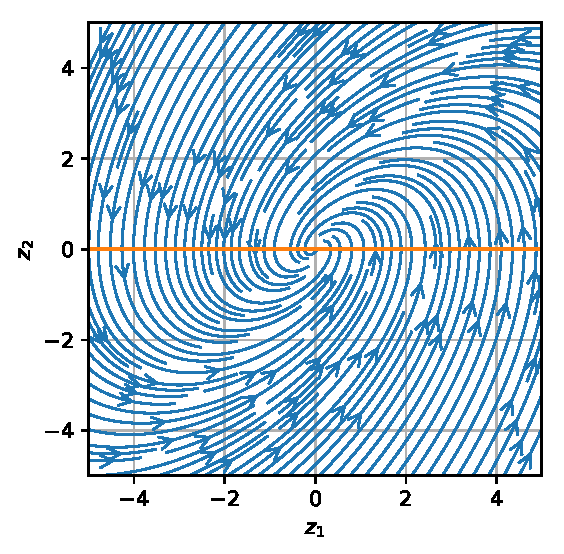
\includegraphics[width = 5cm]{LaSalle2019.pdf}
        \par}
        
 $\dot{V}$ ist genau dann 0, wenn $z_2 = 0$ ist.
        
    \end{solution}
    \item Zeigen Sie, dass $\dot{V}\left(z_{1}, z_{2}\right) \leq 0$ gilt und beurteilen Sie unter Verwendung der Ergebnisse aus Punkt iii die Stabilität der Ruhelage des nichtlinearen Systems.
    \begin{solution}
        $\dot{V}$ ist negativ semidefinit (siehe $\dot{V}$ im Unterpunkt iii). Das nichtlineare System ist jedenfals stabil im Sinne von Ljapunov.
        
        Setzt man $z_2 = 0$ erhält man folgende Gleichungen für das System: 
    
    \[ 
\begin{array}{l}{\dot{z}_{1}=0} \\ {\dot{z}_{2}=z_{1}\left((z_{1}+1)^{2}+1\right)}\end{array}
 \]
 
 Keine Trajektorie verbleibt in $S$ $\rightarrow$ Das System ist asymptotisch stabil.
    \end{solution}
\end{enumerate}
\end{task}
\end{document}